\section{Performance evaluation}
\label{sec:perf_eval}

This section presents an experimental comparison of the seven selected \acrshort{orm} frameworks. The primary goal is to validate the correctness of our previous analysis, measure performance, and assess how effectively each framework integrates into the .NET through its supported query language.

For each framework, we create a set of unit tests performing pre-selected queries. They should cover different areas of querying through \acrshort{orm}(s), such as entity mapping, relationships, result modification, and aggregation.

Notify that we only test read, i.e., \texttt{SELECT}, queries. Those cover a sufficiently large area of features and provide us with enough information to get some insight on capabilities and performance. Other non-read operations, including insert, update, and delete queries, could be explored in future work.

\subsection{Dataset and database}
\label{sec:dataset_database}
% https://learn.microsoft.com/en-us/sql/samples/wide-world-importers-what-is?view=sql-server-ver16
To adequately test performance, we need a sufficiently large data set. Microsoft offers pre-made open source datasets.
For this comparison, the Wide World Importers sample database~\cite{microsoftWWI} has been selected.
It contains a diverse set of fictional data about a company Wide World Importers described as ``wholesale novelty goods importer and distributor operating from the San Francisco bay area.''~\cite{microsoftWWI}

The database contains over thirty tables split into four schemas, namely \texttt{Application}, \texttt{Purchasing}, \texttt{Sales}, and \texttt{Warehouse}. For each query, we select a suitable table and columns that can best showcase the desired feature.

% database, docker, test project, .net
The dataset is made for \acrshort{mssql}.\footnote{\acrshort{mssql} is the third most popular database management system as of March 2025 according to DB-Engines Ranking~\cite{DBEngines2025Ranking}. With a score of 788.14, it is behind Oracle (1253.08) and MySQL (988.13). The score takes into account the number of mentions on websites, frequency of technical discussions, number of job offers mentioning the system, relevance in social networks, and other parameters~\cite{DBEnginesRankingMetrics}.}, which represents database system commonly used in .NET applications, where \acrshort{efcore} framework is used.\footnote{All the three products are developed and maintained by Microsoft corporation.}  
Unit tests should be easy to set up and run. Configuring a database can turn into a complicated task. We will create a Docker container running \acrshort{mssql}. The dataset will be loaded on startup. Execution of unit tests will be just a matter of starting the Docker container and running the \texttt{dotnet test} command (or alternatively using Visual Studio Test Explorer). 

\subsection{Selected queries}
\label{sec:selected_queries}
Our goal is to test the query capabilities as broadly as possible. We want to create queries that use different conditions, result modifications, aggregations, relationships between tables, etc. The queries are grouped into categories \textbf{A -- H} by the type of features they test. Table~\ref{tab:queries-sum} provides an overview of each query purpose. In particular, we go over each query and provide an example of what the query should look like in raw \acrshort{sql}. The example can be used to directly query the test database to preview results. The example might be simplified for this text. Unit tests might use a different query language where available.

\begin{table}[H]
\centering
\caption{Benchmark queries}\label{tab:queries-sum}
\begin{tabular}{ll}
\toprule
\textbf{ID} & \textbf{Query Semantics} \\ 
\midrule
\textbf{A1} & Projection -- entity identical to table \\ 
\textbf{A2} & Limited projection -- subset of columns \\ 
\textbf{A3} & Split projection -- one row to multiple entities \\ 
\textbf{A4} & Stored-procedure projection \\ 
\textbf{B1} & Selection over indexed column \\ 
\textbf{B2} & Selection over non-indexed column \\ 
\textbf{B3} & Range filter \\ 
\textbf{B4} & \texttt{IN} list filter \\ 
\textbf{B5} & Text search \\ 
\textbf{B6} & Paging \\ 
\textbf{C1} & Aggregation -- count \\ 
\textbf{C2} & Aggregation -- max \\ 
\textbf{C3} & Aggregation -- sum with expression \\ 
\textbf{D1} & One-to-many relationship\\ 
\textbf{D2} & Many-to-many relationship \\ 
\textbf{D3} & Optional one-to-many relationship \\ 
\textbf{E1} & Sorting with limit \\ 
\textbf{E2} & Distinct projection \\ 
\textbf{F1} & \acrshort{json} object query \\ 
\textbf{F2} & \acrshort{json} array query \\ 
\textbf{G1} & Set union\\ 
\textbf{G2} & Set intersection \\ 
\textbf{H1} & Metadata lookup -- column data type \\ 
\bottomrule
\end{tabular}
\end{table}

\subsubsection{Group A -- Entity projection}
This group will test how well \acrshort{orm} can handle projecting table columns onto a user-defined entity or entities. Queries \textbf{A1}, \textbf{A2}, and \textbf{A3} will fetch one row based on its \textit{identifier}. The measured time and memory allocation will then show the overhead of the \acrshort{orm} framework when mapping data to the resulting entities. Query \textbf{A4} returns a large number of results, so it is the first query that shows us the performance with high-volume data.

\paragraph{Query A1 -- Entity identical to a table}
\label{query:a1}
The query retrieves a table row and map it to an entity with properties identical to table columns. 
Table \texttt{Purchasing.PurchaseOrders} is queried and one item retrieved based on its identifier \texttt{PurchaseOrderId}.

\begin{lstlisting}[language=SQL]
SELECT * FROM Purchasing.PurchaseOrders 
WHERE PurchaseOrderId = 25
\end{lstlisting}

\paragraph{Query A2 -- Subset of columns}
\label{query:a2}
The resulting entity has fewer properties than table columns. Only the data we really need should be transferred. 
Table \texttt{Purchasing.Suppliers} is queried, and only columns related to the supplier's contact info are retrieved.

\begin{lstlisting}[language=SQL]
SELECT SupplierID, SupplierName, PhoneNumber, FaxNumber, WebsiteURL, ValidFrom, ValidTo 
FROM Purchasing.Suppliers 
WHERE SupplierID = 10
\end{lstlisting}

\paragraph{Query A3 -- One row to multiple entities}
\label{query:a3}
Single table is queried and the resultis divided into two different entities. 
Table \texttt{Purchasing.Suppliers} is used again, from which we retrieve contact information and bank account information into two separate entities. 

\begin{lstlisting}[language=SQL]
SELECT 
    SupplierId, SupplierName, PhoneNumber, FaxNumber, WebsiteURL, ValidFrom, ValidTo, 
    SupplierId, BankAccountName, BankAccountBranch, BankAccountCode, BankAccountNumber, BankInternationalCode 
FROM Purchasing.Suppliers 
WHERE SupplierID = 10
\end{lstlisting}

\paragraph{Query A4 -- Stored procedure result projection}
\label{query:a4}
This query executes a stored procedure, limited by parameters, and loads the result into an entity.
The executed stored procedure is \texttt{Integration.GetOrderUpdates} with parameters \texttt{LastCutoff} and \texttt{NewCutoff}. 
We limit the cut-off to a one-year range from 2014 to 2015. 66741 order updates should be returned.

This stored procedure returns columns with spaces in their names, for example, ``WWI Order ID''. As properties in the C\# language cannot contain spaces, it is interesting to see how and if different frameworks can handle this.

\begin{lstlisting}[language=SQL]
EXEC WideWorldImporters.Integration.GetOrderUpdates 
@LastCutoff = '2014-01-01', @NewCutoff = '2015-01-01'
\end{lstlisting}

\subsubsection{Group B -- Selection}
Probably the most common query operation is limiting results based on a condition (i.e., filtering). This set of queries queries table \texttt{Sales.OrderLines} with varied conditions.

\paragraph{Query B1 -- Selection over indexed column}
\label{query:b1}
The query retrieves one order line based on the identifier \texttt{OrderId}. The identifier is a foreign key with an index built over it.

\begin{lstlisting}[language=SQL]
SELECT * FROM Sales.OrderLines WHERE OrderID = 26866
\end{lstlisting}

\paragraph{Query B2 -- Selection over non-indexed column}
\label{query:b2}
Unlike the first query, this one fetches order lines filtered by a column without an index. The column that we filter over is the unit price of the order line.
It is worth noting that it should not be relevant if a column is indexed or not for \acrshort{orm} comparison. Because all the queries are performed over the same database system. We include both queries in case an interesting result appears.

\begin{lstlisting}[language=SQL]
SELECT * FROM Sales.OrderLines WHERE UnitPrice = 25
\end{lstlisting}

\paragraph{Query B3 -- Range filter}
\label{query:b3}
The previous queries filtered based on a single value, but a range of values is often desirable as well.
This query selects a subset of order lines with a column \texttt{PickingCompletedWhen} within a selected date range.

\begin{lstlisting}[language=SQL]
SELECT * FROM Sales.OrderLines 
WHERE PickingCompletedWhen 
BETWEEN '2014-12-20' AND '2014-12-31'
\end{lstlisting}

\paragraph{Query B4 -- IN list filter}
\label{query:b4}
When a range is not sufficient and we want specific values not fitting into an interval, we can provide a collection of values.
This query will return order lines belonging to orders with \texttt{OrderId} equal to '1', '10', '100', '1000', or '10000'.

\begin{lstlisting}[language=SQL]
SELECT * FROM Sales.OrderLines 
WHERE OrderID IN (1, 10, 100, 1000, 10000)
\end{lstlisting}

\paragraph{Query B5 -- Text search}
\label{query:b5}
This query tests a text search, looking for any order lines with descriptions containing the word ``C++''.  The column does not have a full-text search or any other index.

\begin{lstlisting}[language=SQL]
SELECT * FROM Sales.OrderLines 
WHERE Description LIKE '%C++%'
\end{lstlisting}

\paragraph{Query B6 -- Paging}
\label{query:b6}
When filtering with a broad condition, a large amount of data might be returned. So we may opt to receive the data in batches. Another use case might be a paged table displayed to a user. For these, a paging query with skip and take might be useful.
This query fetches all order lines ordered by identifier, but will skip the first 1000 rows and take only the next 50 rows.

\begin{lstlisting}[language=SQL]
SELECT * FROM Sales.OrderLines 
ORDER BY OrderLineID 
OFFSET 1000 ROWS FETCH NEXT 50 ROWS ONLY
\end{lstlisting}

\subsubsection{Group C -- Aggregation}
Aggregation functions are often used when performing calculations on data. In this group, we test a selected sample of them.

\paragraph{Query C1 -- Count}
\label{query:c1}
Count is very useful when we need to know the number of records that correspond to a specific condition. We combine it with \texttt{GROUP BY} clause to retrieve distinct tax rates and the number of their occurrences.

\begin{lstlisting}[language=SQL]
SELECT TaxRate, COUNT(TaxRate) as Count 
FROM Sales.OrderLines 
GROUP BY TaxRate 
ORDER BY Count DESC
\end{lstlisting}

\paragraph{Query C2 -- Max}
\label{query:c2}
Maximum and minimum are also commonly used. We attempt to retrieve the maximum unit price for all order lines.

\begin{lstlisting}[language=SQL]
SELECT MAX(UnitPrice) FROM Sales.OrderLines
\end{lstlisting}

\paragraph{Query C3 -- Sum}
\label{query:c3}
Aggregation functions also allow performing operations. In this test, we combine the \texttt{SUM} function with a multiplication inside. The result is the total price across all order lines.

\begin{lstlisting}[language=SQL]
SELECT SUM(Quantity * UnitPrice) FROM Sales.OrderLines
\end{lstlisting}

\subsubsection{Group D -- Relations}
An important feature of \acrshort{orm} should be mapping relations. Our domain entities are often connected, representing relations in real life.
However, as we found out in our previous analysis, not all the selected frameworks support mapping relations. 

Our test data contain no one-to-one relation. There should be a small difference between mapping one-to-one and one-to-many. We cover the other types in sufficient detail.

Some \acrshort{orm}(s) support lazy loading, i.e., loading entities in a relation only after accessing the corresponding collection. That would result in more queries being sent and a potential slowdown.
We prevent this by setting the loading strategy to eager when possible.

\paragraph{Query D1 -- One-to-many}
\label{query:d1}
In a one-to-many relation, we have one parent and multiple children. A parent entity should have a collection containing its children. Optionally, a child entity can have a reference to its parent.
In this test, we use the relation between an order and its order lines. We fetch one specific order along with all its lines.

We need to verify all child entities were returned and the parent collection filled. 

\begin{lstlisting}[language=SQL]
SELECT o.*, ol.* FROM Sales.Orders o
LEFT JOIN Sales.OrderLines ol ON ol.OrderID = o.OrderID
WHERE o.OrderID = 530
\end{lstlisting}

\paragraph{Query D2 -- Many-to-many}
\label{query:d2}
In a many-to-many relation, both sides can be connected with multiple entities of the same type. Therefore, it will be represented by a collection on both sides. The collection can contain the entity directly, which makes it easier for developers to work with. If necessary, it can contain entities that represent the join table for this relationship.

This test consists of two queries. We want to test accessing the relationship from both sides. The first query fetches stock items with their stock groups. And the other one stock groups with their stock items.
The relationship is represented by a join table \texttt{Warehouse.StockItemStockGroups}. If possible, we try to map this relation without a join entity in our tests.

\begin{lstlisting}[language=SQL]
SELECT si.*, sg.* FROM Warehouse.StockItems si
LEFT JOIN Warehouse.StockItemStockGroups sisg
    ON si.StockItemID = sisg.StockItemID
LEFT JOIN Warehouse.StockGroups sg
    ON sisg.StockGroupID = sg.StockGroupID
ORDER BY si.StockItemID
\end{lstlisting}
\begin{lstlisting}[language=SQL]
 SELECT sg.*, si.* FROM Warehouse.StockGroups sg
 LEFT JOIN Warehouse.StockItemStockGroups sisg
     ON sg.StockGroupID = sisg.StockGroupID
 LEFT JOIN Warehouse.StockItems si
     ON sisg.StockItemID = si.StockItemID
 ORDER BY sg.StockGroupID
\end{lstlisting}

Note that the queries utilise left join, so we get all stock items, even if they belong to no stock groups. And vice versa for the other query.

\paragraph{Query D3 -- Optional one-to-many relationship}
\label{query:d3}
In test case \hyperref[query:d1]{D1}, the one-to-many relation was not optional. Each order has at least one order line. In test case \hyperref[query:d2]{D2}, each item belonged to at least one category as well. In contrary to previous cases, this test case utilizes an optional one-to-many relation between a customer and a transaction. 

\begin{lstlisting}[language=SQL]
SELECT c.*, ct.* FROM Sales.Customers c
LEFT JOIN Sales.CustomerTransactions ct
    ON c.CustomerID = ct.CustomerID
ORDER BY c.CustomerID
\end{lstlisting}

\subsubsection{Group E -- Result modification}
This category tests modifying the result set. We test sorting by a column and filtering distinct result values.

\paragraph{Query E1 -- Sorting with limit}
\label{query:e1}
Although we have used sorting to order the results of some previous tests to get deterministic results, this test focuses solely on sorting.
We sort all purchase orders by their expected delivery date and retrieve only the first one thousand.

\begin{lstlisting}[language=SQL]
SELECT TOP (1000) * FROM Purchasing.PurchaseOrders 
ORDER BY ExpectedDeliveryDate ASC
\end{lstlisting}

\paragraph{Query E2 -- Distinct projection}
\label{query:e2}
To test fetching only unique values, we request all supplier references from purchase orders.

\begin{lstlisting}[language=SQL]
SELECT DISTINCT SupplierReference 
FROM Purchasing.PurchaseOrders
\end{lstlisting}

\subsubsection{Group F -- JSON queries}
\acrshort{mssql} supports storing and querying \acrshort{json} data~\cite{mssqljson}. It is worth testing if our selected \acrshort{orm}(s) support constructing queries into the stored \acrshort{json}.
Table \texttt{Application.People} contains text columns storing \acrshort{json} values.

During the static comparison, we found that none of the selected \acrshort{orm}(s) supports \acrshort{xml} or any other data format, therefore we do not cover for those.

\paragraph{Query F1 -- JSON object query}
\label{query:f1}
Column \texttt{CustomFields} contains a \acrshort{json} with many different values. In this test, we focus on property \texttt{Title}. We query all people with a title set to ``Team Member''.
We accomplish that using the \texttt{JSON\_VALUE} \acrshort{sql} function.

\begin{lstlisting}[language=SQL]
SELECT * FROM Application.People
WHERE JSON_VALUE(CustomFields, '$.Title') = 'Team Member'
ORDER BY PersonId
\end{lstlisting}

\paragraph{Query F2 -- JSON array query}
\label{query:f2}
The first case covered querying a \acrshort{json} object. This one tests querying inside a \acrshort{json} array. Column \texttt{OtherLanguages} contains a \acrshort{json} array containing language names.

\begin{lstlisting}[language=SQL]
SELECT * FROM Application.People
WHERE EXISTS (
    SELECT 1
    FROM OPENJSON(OtherLanguages)
    WHERE value = 'Slovak'
)
\end{lstlisting}

\subsubsection{Group G -- Set operations}
In the last group we will test common set operations. Those are useful when having to combine two sets of data.

\paragraph{Query G1 -- Union}
\label{query:g1}
Union combines results from both queries. In this test, we combine results from two different intervals of IDs and ensure that they are all present in the result.

\begin{lstlisting}[language=SQL]
SELECT SupplierID FROM Purchasing.Suppliers 
    WHERE SupplierID < 5
UNION
SELECT SupplierID FROM Purchasing.Suppliers 
    WHERE SupplierID BETWEEN 5 AND 10
ORDER BY SupplierID
\end{lstlisting}

\paragraph{Query G2 -- Intersection}
\label{query:g2}
Intersection includes results that appear in both of the queries. We try combining supplier IDs in two overlapping intervals and assert that only the overlap is included. 

\begin{lstlisting}[language=SQL]
SELECT SupplierID FROM Purchasing.Suppliers 
    WHERE SupplierID < 10
INTERSECT
SELECT SupplierID FROM Purchasing.Suppliers 
    WHERE SupplierID BETWEEN 5 AND 15
ORDER BY SupplierID
\end{lstlisting}

\subsubsection{Group H -- Metadata lookup}
In the last section, we briefly test the \acrshort{orm} framework's ability to query information about the database itself. While not commonly used in applications, such data can be required in specific cases.

\paragraph{Query H1 -- Column data type}
\label{query:h1}
The final query attempts to retrieve the data type of a table column. All information about the database schema is available through \texttt{INFORMATION\_SCHEMA.COLUMNS} table. The selected column has \texttt{NVARCHAR} type. Note that the table contains information such as nullability, or maximum length, but for demonstration purposes, a simple query returning only data type should be sufficient.

\begin{lstlisting}[language=SQL]
SELECT DATA_TYPE FROM INFORMATION_SCHEMA.COLUMNS 
WHERE TABLE_SCHEMA = 'Purchasing'
    AND TABLE_NAME = 'Suppliers'
    AND COLUMN_NAME = 'SupplierReference'
\end{lstlisting}

\subsubsection{Summary of the selected queries}
We tried to pick as broad a selection of features as possible. 
The set is not exhaustive but representative enough to give us a fair idea of how different \acrshort{orm}(s) perform. 

The tests perform queries across different tables and fetch different amounts of data. 
Measured time and memory allocation will not allow us to make any assumptions when comparing different test cases for the same \acrshort{orm}.
But we will be able to compare identical test cases across different \acrshort{orm}(s).

We can expect to see a difference in time performance between micro frameworks made to be efficient and feature-rich macro frameworks.
The micro frameworks utilize raw \acrshort{sql} and have very little overhead. When using a macro framework, the \acrshort{linq} query has to be compiled into \acrshort{sql}. Rich mapping capabilities may also cause significant slowdown. And extra features may even cause higher memory consumption.

\subsection{Testing approach}
\label{sec:testing_approach}
We prefer to use \acrshort{linq} where possible as it is tightly integrated into the .NET environment. 
If \acrshort{linq} integration is not available, we use any suitable alternative. And if there are no other possibilities, we default to raw \acrshort{sql} queries. 

There are multiple different methods for mapping database tables to entities. We use different methods to show the variety and their impact or trade-offs. 

If \acrshort{orm} supports caching entities, we disable it so that our benchmarks are not affected. 
A feature related to caching is change tracking. For example, \acrshort{efcore} tracks changes made to an entity, so that it can later perform an update. All our tests will only execute read operations. Change tracking would unnecessarily increase measured time or allocated memory, so we will disable it.

Logging is turned off for performance tests. In feature tests, we might want to compare generated \acrshort{sql}. So, we enable \acrshort{sql} logging into the test output window where possible.

To showcase different approaches to mapping, we try to select a different method for each framework test. Mapping is usually compiled on application startup or the first query and then cached. So performance should not be affected by a choice of mapping. Dapper does not use any mapping. PetaPoco and RepoDB use attributes to declare table schema and name, and in some cases column names; the rest is inferred. LINQ to DB utilizes mapping by code through the builder pattern. NHibernate uses its proprietary mapping through files in \acrshort{xml} format. Both versions of Entity Framework use attribute mapping combined with mapping through code. Their attribute mapping is much more powerful than those of PetaPoco and RepoDB, but in more complex cases, mapping by code has to be supplied.

\subsection{Implementation}
The comparison was implemented in the form of a Visual Studio solution, containing a project folder for each framework. Each project folder contains three projects -- entities, feature tests, and performance benchmark. 

\begin{figure}[h!]
\usetikzlibrary{positioning, arrows}
\begin{center}
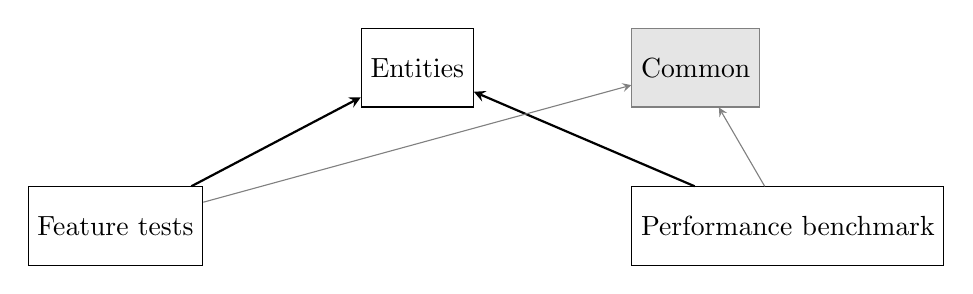
\begin{tikzpicture}[
    node distance=1cm and 2cm,
    every node/.style={draw, minimum width=1cm, minimum height=1cm, align=center},
    every path/.style={->, >=stealth},
    faded/.style={draw=gray, fill=gray!20},
    faded_arrow/.style={->, >=stealth, draw=gray}
]

  \node (E) {Entities};
  \node (C) [right=of E, faded] {Common};
  \node (FT) [below left=of E] {Feature tests};
  \node (PB) [below right=of E] {Performance benchmark};

  \draw[thick, ->, >=stealth] (FT) -- (E);
  \draw[thick, ->, >=stealth] (PB) -- (E);
  \draw[faded_arrow] (FT) -- (C);
  \draw[faded_arrow] (PB) -- (C);

\end{tikzpicture}
\end{center}
    
    \caption{Caption}
    \label{fig:enter-label}
\end{figure}

Common project is also included. It contains a single class handling loading the database connection string from a configuration file. There is no dependency between feature tests and performance tests. It could be argued that the code for queries could be extracted to a separate class to avoid duplication. But we have kept it duplicated to isolate unit tests from performance benchmarks. This structure is repeated for each of the seven frameworks we are examining. There is again no dependency between the different frameworks for isolation purposes.

\subsubsection{Technology overview}
As we have decided before implementation in Section~\autoref{sec:dataset_database}, we are using \acrshort{mssql} with World Wide Importers data set. The database system is running in a Docker container. Base image used is \texttt{mssql/server:2022-latest}~\cite{mssqlDocker} provided by Microsoft. The image imports our dataset and waits until it is ready.

The .NET tests are structured in .NET projects grouped in one solution. .NET version 8 was chosen as it is the latest long term support (\acrshort{lts}) version at the time of writing~\cite{NETversions}. Tests are developed and run using Microsoft Visual Studio 2022, but \texttt{dotnet} \acrshort{cli} commands are provided as well.

\subsubsection{Installation instructions}
The container was tested both in Docker\footnote{\url{https://docs.docker.com/}} and Podman\footnote{\url{https://podman.io/docs}}. A \texttt{Dockerfile} is provided in \texttt{benchmarks/Dockerfile}. Container image can be built and started using the two commands below. Replace \texttt{'docker'} with \texttt{'podman'} if needed. The database system will be exposed on port 1444, under username \texttt{'SA'} and password \texttt{'Testingorms123'}.
The third command can be used to test connection. The \texttt{sqlcmd} utility is available only if you have \acrshort{mssql} installed locally. Otherwise, use any database management tool of your choice.

\begin{lstlisting}[language=sh]
docker build -t orm-comparison .

docker run -d --name orm-comparison -p 1444:1433 orm-comparison

sqlcmd -S 127.0.0.1,1444 -U SA -P Testingorms123 -Q "SELECT * FROM [WideWorldImporters].[Purchasing].[PurchaseOrders]"
\end{lstlisting}

To run feature unit tests, build the project in Visual Studio and then use the Test Explorer window to select and run specific tests. Alternatively, navigate to the folder with the solution file and run \lstinline{dotnet test}. This will build the project, find all tests, and run them. 

To run performance benchmarks, set \texttt{BenchmarkMain} as a startup project. Right-click it in the Solution Explorer window and choose \textit{'Set as Startup project'}. Make sure configuration is set to Release, not Debug. Then start the project without debugging (\texttt{CTRL + F5} keys). A console window will appear. It contains instructions on how to target specific benchmarks. To run all, type in an asterisk (\texttt{'*'}) and press enter. This will trigger a full run, which takes approximately one hour to finish. You can switch to the test configuration which does only a few numbers of iterations in \texttt{BenchmarkMain/Program.cs} file. What the configuration does is further explained in the following sections. 

Console command for running benchmarks is \lstinline{dotnet run --configuration Release --project BenchmarkMain\BenchmarkMain.csproj}. To run with a shorter test configuration, append \lstinline{-- --testb} at the end of the command.

\subsubsection{Feature tests}
For each query defined in Section~\ref{sec:selected_queries}, a unit test in the form of an isolated method was implemented. Connection and other configuration are created outside of the test in a setup part. The method executes the query and correct results are asserted. Assertion checks the amount of results and their order. Each property is tested to contain correct data to ensure mapping was done correctly.

The example below shows Query A1 (see Section~\ref{query:a1}) implemented for Dapper. A single purchase order is retrieved based on its ID, and its properties are checked for correct values. 
\begin{lstlisting}[language=CSharp]
[Fact]
public void A1_EntityIdenticalToTable()
{
    var order = connection.QuerySingle<PurchaseOrder>(
        "SELECT * FROM WideWorldImporters.Purchasing.PurchaseOrders WHERE PurchaseOrderId = @PurchaseOrderId",
        new { PurchaseOrderId = 25 }
    );

    Assert.Multiple(() =>
    {
        Assert.Equal(25, order.PurchaseOrderID);
        Assert.Equal(12, order.SupplierID);
        Assert.Equal(new DateTime(2013, 1, 5), order.OrderDate);
        ...
    });
}
\end{lstlisting}

As decided in Section~\ref{sec:testing_approach}, we have attempted to use \acrshort{linq} query language. Where not supported we have used any available alternative that did not involve just writing raw \acrshort{sql}. And finally, where nothing else was possible we have used the raw alternative to have a passing test.  
%TODO mention the table that will have feature comparison

\subsubsection{Performance benchmarks}
Feature tests can assert the correctness of returned results and overall functionality. But their execution time can greatly vary. There can be some overhead, coming from test initialization or assertions. The system the benchmarks are running on can also impact results.

To solve these problems we have used BenchmarkDotNet library~\cite{BenchmarkDotNet}. It allows writing benchmark methods very similar to unit tests. In fact, they are completely identical to unit tests, the only differences are missing assertions and a different method attribute. It allows us to ``transform methods into benchmarks, track their performance, and share reproducible measurement experiments''~\cite{BenchmarkDotNet}. Work with the library was quite easy, it is very configurable and easy to run. 

It runs benchmark for each method multiple times. It starts with a few iterations which will not be included in the results. The first few ensure \textit{just-in-time} (\acrshort{jit}) compilation has taken effect, then multiple iterations without actually running the method code are started to compile overhead. The overhead is removed from the results, ensuring reliability. 

According to BenchmarkDotNet documentation~\cite{BenchmarkDotNetHow}, a single benchmark run consists of the following stages:
\begin{itemize}
    \item \textit{OverheadJitting} -- Measures benchmarking infrastructure compilation.
    \item \textit{WorkloadJitting} -- Measures benchmark method compilation.
    \item \textit{WorkloadPilot} -- Selects best iteration count based on heuristics.
    \item \textit{WorkloadWarmup} -- Runs several iterations before measuring to ensure factors like \acrshort{cpu} caching or branch prediction are optimized.
    \item \textit{WorkloadActual} -- Actual measurements
    \item \textit{WorkloadResult} -- Result calculated from the actual run without the overhead.
\end{itemize}

After the benchmark run finishes, results and run log can be found in folder \path{benchmarks/BenchmarkMain/bin/Release/net8.0/} saved in file \path{BenchmarkDotNet.Artifacts}.

\smallskip
The referenced run results are copied to \path{benchmarks/results/joined}.

\smallskip
Notable result files include:
\begin{itemize}
    \item \path{BenchmarkRun-joined-2025-03-06-16-10-18-report.csv}\\
    Measurements of all benchmarks in \acrshort{csv} format.

    \item \path{BenchmarkRun-joined-2025-03-06-16-10-18-report.html}\\
    Summary table of all benchmarks (\acrshort{html} format).

    \item \path{BenchmarkRun-joined-2025-03-06-16-10-18-report-github.md}\\
    Summary table of all benchmarks (Markdown format suitable for GitHub).

    \item \path{BenchmarkRun-joined-2025-03-06-16-10-18-measurements.csv}\\
    Detailed measurements of every single iteration of each benchmark.
\end{itemize}

\subsection{Interpretation of results}
Results are accompanied by tables showing results across all test cases. 

Table~\ref{tab:feature_comp} summarizes feature test outcomes. The base result indicates if the query could be expressed within each framework (\texttt{'Y'} = yes, \texttt{'N'} = no). Outcomes are categorized as:
\begin{itemize}
    \item \textbf{Y LINQ}: \acrshort{linq} fully supported.
    \item \textbf{Y lambda expr.}: Supported using lambda expressions, less expressive than \acrshort{linq}.
    \item \textbf{Y raw SQL}: Query had to be written directly in \acrshort{sql}, either in string or using a builder.
    \item \textbf{N manually in memory}: Query required manual post-computation in memory.
    \item \textbf{N custom JSON parsing/converter}: \acrshort{json} could not be queried and had to be parsed in memory.
    \item \textbf{N error}: Query failed with exception that could not be fixed. 
\end{itemize}
The negative results are discussed in detail further in the subsequent text.

\afterpage{
\begin{landscape}
\begin{table}[htp]
\centering
\caption{Feature comparison}
\label{tab:feature_comp}
\scriptsize
\begin{threeparttable}[!htb]
\def\arraystretch{1.25}
\begin{tabular}{
>{\raggedright\arraybackslash}p{50.00mm}
>{\raggedright\arraybackslash}p{20.00mm}
>{\raggedright\arraybackslash}p{20.00mm}
>{\raggedright\arraybackslash}p{20.00mm}
>{\raggedright\arraybackslash}p{20.00mm}
>{\raggedright\arraybackslash}p{20.00mm}
>{\raggedright\arraybackslash}p{20.00mm}
>{\raggedright\arraybackslash}p{20.00mm}
>{\raggedright\arraybackslash}p{20.00mm}
}
\toprule
\textbf{Benchmark Name} & \textbf{Dapper} & \textbf{PetaPoco} & \textbf{RepoDB} & \textbf{linq2db} & \textbf{NHibernate} & \textbf{EF6} & \textbf{EF Core} \\
\midrule
A1\_EntityIdenticalToTable &Y raw SQL &Y raw SQL &\cellcolor[HTML]{d9ead3}Y lambda expr. &\cellcolor[HTML]{b7e1cd}Y LINQ &\cellcolor[HTML]{b7e1cd}Y LINQ &\cellcolor[HTML]{b7e1cd}Y LINQ &\cellcolor[HTML]{b7e1cd}Y LINQ \\
A2\_LimitedEntity &Y raw SQL &Y raw SQL &\cellcolor[HTML]{d9ead3}Y lambda expr. &\cellcolor[HTML]{b7e1cd}Y LINQ &\cellcolor[HTML]{b7e1cd}Y LINQ &\cellcolor[HTML]{b7e1cd}Y LINQ &\cellcolor[HTML]{b7e1cd}Y LINQ \\
A3\_MultipleEntitiesFromOneResult &Y raw SQL &Y raw SQL &\cellcolor[HTML]{d9ead3}Y lambda expr. &\cellcolor[HTML]{b7e1cd}Y LINQ &\cellcolor[HTML]{b7e1cd}Y LINQ &\cellcolor[HTML]{b7e1cd}Y LINQ &\cellcolor[HTML]{b7e1cd}Y LINQ \\
A4\_StoredProcedureToEntity &Y raw SQL &Y raw SQL &Y raw SQL &Y raw SQL &\cellcolor[HTML]{ea9999}N error &\cellcolor[HTML]{ea9999}N error &Y raw SQL \\
B1\_SelectionOverIndexedColumn &Y raw SQL &Y raw SQL &\cellcolor[HTML]{d9ead3}Y lambda expr. &\cellcolor[HTML]{b7e1cd}Y LINQ &\cellcolor[HTML]{b7e1cd}Y LINQ &\cellcolor[HTML]{b7e1cd}Y LINQ &\cellcolor[HTML]{b7e1cd}Y LINQ \\
B2\_SelectionOverNonIndexedColumn &Y raw SQL &Y raw SQL &\cellcolor[HTML]{d9ead3}Y lambda expr. &\cellcolor[HTML]{b7e1cd}Y LINQ &\cellcolor[HTML]{b7e1cd}Y LINQ &\cellcolor[HTML]{b7e1cd}Y LINQ &\cellcolor[HTML]{b7e1cd}Y LINQ \\
B3\_RangeQuery &Y raw SQL &Y raw SQL &\cellcolor[HTML]{d9ead3}Y lambda expr. &\cellcolor[HTML]{b7e1cd}Y LINQ &\cellcolor[HTML]{b7e1cd}Y LINQ &\cellcolor[HTML]{b7e1cd}Y LINQ &\cellcolor[HTML]{b7e1cd}Y LINQ \\
B4\_InQuery &Y raw SQL &Y raw SQL &\cellcolor[HTML]{d9ead3}Y lambda expr. &\cellcolor[HTML]{b7e1cd}Y LINQ &\cellcolor[HTML]{b7e1cd}Y LINQ &\cellcolor[HTML]{b7e1cd}Y LINQ &\cellcolor[HTML]{b7e1cd}Y LINQ \\
B5\_TextSearch &Y raw SQL &Y raw SQL &\cellcolor[HTML]{d9ead3}Y lambda expr. &\cellcolor[HTML]{b7e1cd}Y LINQ &\cellcolor[HTML]{b7e1cd}Y LINQ &\cellcolor[HTML]{b7e1cd}Y LINQ &\cellcolor[HTML]{b7e1cd}Y LINQ \\
B6\_PagingQuery &Y raw SQL &Y raw SQL &\cellcolor[HTML]{d9ead3}Y lambda expr. &\cellcolor[HTML]{b7e1cd}Y LINQ &\cellcolor[HTML]{b7e1cd}Y LINQ &\cellcolor[HTML]{b7e1cd}Y LINQ &\cellcolor[HTML]{b7e1cd}Y LINQ \\
C1\_AggregationCount &Y raw SQL &Y raw SQL &\cellcolor[HTML]{f4cccc}N manually in memory &\cellcolor[HTML]{b7e1cd}Y LINQ &\cellcolor[HTML]{b7e1cd}Y LINQ &\cellcolor[HTML]{b7e1cd}Y LINQ &\cellcolor[HTML]{b7e1cd}Y LINQ \\
C2\_AggregationMax &Y raw SQL &Y raw SQL &\cellcolor[HTML]{d9ead3}Y lambda expr. &\cellcolor[HTML]{b7e1cd}Y LINQ &\cellcolor[HTML]{b7e1cd}Y LINQ &\cellcolor[HTML]{b7e1cd}Y LINQ &\cellcolor[HTML]{b7e1cd}Y LINQ \\
C3\_AggregationSum &Y raw SQL &Y raw SQL &Y raw SQL &\cellcolor[HTML]{b7e1cd}Y LINQ &\cellcolor[HTML]{b7e1cd}Y LINQ &\cellcolor[HTML]{b7e1cd}Y LINQ &\cellcolor[HTML]{b7e1cd}Y LINQ \\
D1\_OneToManyRelationship &\cellcolor[HTML]{f4cccc}N manually in memory &\cellcolor[HTML]{f4cccc}N manually in memory &\cellcolor[HTML]{d9ead3}Y lambda expr. &\cellcolor[HTML]{b7e1cd}Y LINQ + mapping &\cellcolor[HTML]{b7e1cd}Y LINQ + mapping &\cellcolor[HTML]{b7e1cd}Y LINQ + mapping &\cellcolor[HTML]{b7e1cd}Y LINQ + mapping \\
D2\_ManyToManyRelationship &\cellcolor[HTML]{f4cccc}N manually in memory &\cellcolor[HTML]{f4cccc}N manually in memory &\cellcolor[HTML]{f4cccc}N manually in memory &\cellcolor[HTML]{b7e1cd}Y LINQ + mapping, join entity &\cellcolor[HTML]{b7e1cd}Y LINQ + mapping &\cellcolor[HTML]{b7e1cd}Y LINQ + mapping &\cellcolor[HTML]{b7e1cd}Y LINQ + mapping \\
D3\_OptionalRelationship &\cellcolor[HTML]{f4cccc}N manually in memory &\cellcolor[HTML]{f4cccc}N manually in memory &\cellcolor[HTML]{d9ead3}Y lambda expr. &\cellcolor[HTML]{b7e1cd}Y LINQ + mapping &\cellcolor[HTML]{b7e1cd}Y LINQ + mapping &\cellcolor[HTML]{b7e1cd}Y LINQ + mapping &\cellcolor[HTML]{b7e1cd}Y LINQ + mapping \\
E1\_ColumnSorting &Y raw SQL &Y raw SQL &\cellcolor[HTML]{d9ead3}Y lambda expr. &\cellcolor[HTML]{b7e1cd}Y LINQ &\cellcolor[HTML]{b7e1cd}Y LINQ &\cellcolor[HTML]{b7e1cd}Y LINQ &\cellcolor[HTML]{b7e1cd}Y LINQ \\
E2\_Distinct &Y raw SQL &Y raw SQL &Y raw SQL &\cellcolor[HTML]{b7e1cd}Y LINQ &\cellcolor[HTML]{b7e1cd}Y LINQ &\cellcolor[HTML]{b7e1cd}Y LINQ &\cellcolor[HTML]{b7e1cd}Y LINQ \\
F1\_NestedJSONQuery &\cellcolor[HTML]{f4cccc}N custom JSON parsing &\cellcolor[HTML]{f4cccc}N custom JSON parsing &\cellcolor[HTML]{f4cccc}N custom JSON parsing &\cellcolor[HTML]{f4cccc}N custom converter &\cellcolor[HTML]{f4cccc}N custom JSON parsing &\cellcolor[HTML]{f4cccc}N custom JSON parsing &\cellcolor[HTML]{b7e1cd}Y LINQ \\
F2\_JSONArrayQuery &\cellcolor[HTML]{f4cccc}N custom JSON parsing &\cellcolor[HTML]{f4cccc}N custom JSON parsing &\cellcolor[HTML]{f4cccc}N custom JSON parsing &\cellcolor[HTML]{f4cccc}N custom converter &\cellcolor[HTML]{f4cccc}N custom JSON parsing &\cellcolor[HTML]{f4cccc}N custom JSON parsing &\cellcolor[HTML]{b7e1cd}Y LINQ \\
G1\_Union &Y raw SQL &Y raw SQL &Y raw SQL &\cellcolor[HTML]{b7e1cd}Y LINQ &\cellcolor[HTML]{b7e1cd}Y LINQ &\cellcolor[HTML]{b7e1cd}Y LINQ &\cellcolor[HTML]{b7e1cd}Y LINQ \\
G2\_Intersection &Y raw SQL &Y raw SQL &Y raw SQL &\cellcolor[HTML]{b7e1cd}Y LINQ &\cellcolor[HTML]{b7e1cd}Y LINQ &\cellcolor[HTML]{b7e1cd}Y LINQ &\cellcolor[HTML]{b7e1cd}Y LINQ \\
H1\_Metadata &Y raw SQL &Y raw SQL &Y raw SQL &Y raw SQL &Y raw SQL &Y raw SQL &Y raw SQL \\
\bottomrule
\end{tabular}
\end{threeparttable}
\end{table}
\end{landscape}
}

Table~\ref{tab:benchmark_results_time} presents measured execution time (in microseconds), and Table~\ref{tab:benchmark_results_memory} presents allocated memory during the run of the benchmark. Reported numbers in text will be rounded to the nearest integer.

Performance tests have to be considered in the context of the feature test results. It was not possible to write all tests in the same way across all frameworks. In some cases, pure ADO.NET queries were used when the framework failed entirely. Additionally, some queries required additional processing in memory, significantly affecting memory usage. These anomalies will be explicitly noted.

Certain frameworks cannot log generated \acrshort{sql} statements to console or file. For those, Microsoft SQL Server Profiler~\cite{sqlProfiler} was used. It allows capturing of any event happening in the Microsoft SQL Server database, including incoming \acrshort{sql} queries. That makes us able to inspect the raw query after it leaves our application and the frameworks can make no further edits to it.

\afterpage{
\begin{landscape}
\begin{table}
\centering
\caption{Performance benchmark results - Mean time (\unit{\micro\second})}
\label{tab:benchmark_results_time}
\scriptsize
\def\arraystretch{1.50}
\begin{tabular}{
>{\raggedright\arraybackslash}p{50.00mm}
>{\raggedleft\arraybackslash}p{20.00mm}
>{\raggedleft\arraybackslash}p{20.00mm}
>{\raggedleft\arraybackslash}p{20.00mm}
>{\raggedleft\arraybackslash}p{20.00mm}
>{\raggedleft\arraybackslash}p{20.00mm}
>{\raggedleft\arraybackslash}p{20.00mm}
>{\raggedleft\arraybackslash}p{20.00mm}
>{\raggedleft\arraybackslash}p{20.00mm}
}
\toprule
\textbf{Namespace} &    \textbf{Dapper} &  \textbf{PetaPoco} &    \textbf{RepoDB} &   \textbf{Linq2db} &  \textbf{NHibernate} &        \textbf{EF6} &     \textbf{EFCore} \\
\midrule
A1\_EntityIdenticalToTable        &      750 &     \cellcolor[HTML]{A1E176} 722 &      748 &      839 &        742 &        \cellcolor[HTML]{FD817B} 854 &        809 \\
A2\_LimitedEntity                 &     \cellcolor[HTML]{A1E176} 718 &      726 &      735 &      858 &       \cellcolor[HTML]{FD817B} 958 &        882 &        799 \\
A3\_MultipleEntitiesFromOneResult &     \cellcolor[HTML]{A1E176} 736 &      \cellcolor[HTML]{A1E176}736 &      745 &      898 &     \cellcolor[HTML]{FD817B} 1 001 &        945 &        832 \\
A4\_StoredProcedureToEntity       &  523 239 & \cellcolor[HTML]{A1E176} 505 967 &  523 242 &  519 491 &   \cellcolor[HTML]{FD817B} 621 739 &    514 077 &    521 573 \\
B1\_SelectionOverIndexedColumn    &     \cellcolor[HTML]{A1E176} 744 &      759 &      762 &      868 &        817 &       \cellcolor[HTML]{FD817B} 905 &        806 \\
B2\_SelectionOverNonIndexedColumn &   43 612 &  \cellcolor[HTML]{A1E176} 41 100 &   43 052 &   43 708 &     86 419 &   \cellcolor[HTML]{FD817B} 125 169 &     48 016 \\
B3\_RangeQuery                    &   30 393 &   29 935 &  \cellcolor[HTML]{FD817B} 30 746 &   21 909 &     22 289 &     22 823 &    \cellcolor[HTML]{A1E176} 21 102 \\
B4\_InQuery                       &      856 &     \cellcolor[HTML]{A1E176} 855 &      876 &      954 &        945 &     \cellcolor[HTML]{FD817B} 1 408 &      1 147 \\
B5\_TextSearch                    & \cellcolor[HTML]{FD817B} 747 728 &  747 721 &  745 551 &  745 319 &    746 464 &    746 264 &   \cellcolor[HTML]{A1E176} 744 754 \\
B6\_PagingQuery                   &    1 327 &   \cellcolor[HTML]{A1E176} 1 314 &    1 556 &    1 458 &      1 447 &     \cellcolor[HTML]{FD817B} 1 710 &      1 406 \\
C1\_AggregationCount              &  \cellcolor[HTML]{A1E176} 35 006 &   35 289 & \cellcolor[HTML]{FD817B} 377 349 &   35 372 &     35 553 &     35 364 &     35 286 \\
C2\_AggregationMax                &    1 240 &  \cellcolor[HTML]{A1E176}  1 227 &    1 264 &   \cellcolor[HTML]{FD817B} 1 380 &      1 291 &      1 366 &      1 304 \\
C3\_AggregationSum                &   86 499 &   85 944 &   86 899 &   86 145 &     75 137 &    \cellcolor[HTML]{A1E176} 69 827 &    \cellcolor[HTML]{FD817B} 87 825 \\
D1\_OneToManyRelationship         &      781 &     \cellcolor[HTML]{A1E176} 770 &      806 &   \cellcolor[HTML]{FD817B} 2 997 &      1 042 &      1 581 &        895 \\
D2\_ManyToManyRelationship        &    4 584 &  \cellcolor[HTML]{A1E176}  4 480 &    6 031 &    9 383 &      5 940 &      6 913 &    \cellcolor[HTML]{FD817B} 14 964 \\
D3\_OptionalRelationship          &  187 693 &  172 030 &  393 631 &  \cellcolor[HTML]{A1E176} 91 326 &    533 489 &  1 993 146 & \cellcolor[HTML]{FD817B} 2 548 411 \\
E1\_ColumnSorting                 &    4 725 &   \cellcolor[HTML]{A1E176} 4 622 &    4 963 &    4 845 &     \cellcolor[HTML]{FD817B} 6 316 &      6 204 &      4 885 \\
E2\_Distinct                      &    2 181 &  \cellcolor[HTML]{A1E176}  2 148 &    2 180 &   \cellcolor[HTML]{FD817B} 2 374 &      2 229 &      2 340 &      2 270 \\
F1\_JSONObjectQuery               &    1 459 &    1 478 &  \cellcolor[HTML]{A1E176}  1 457 &   \cellcolor[HTML]{FD817B} 1 552 &      1 494 &      1 490 &      1 544 \\
F2\_JSONArrayQuery                &    1 723 &   \cellcolor[HTML]{A1E176} 1 718 &    1 732 &    1 795 &      1 761 &      1 771 &     \cellcolor[HTML]{FD817B} 1 839 \\
G1\_Union                         &      728 &    \cellcolor[HTML]{A1E176}  715 &      723 &    1 580 &      1 538 &     \cellcolor[HTML]{FD817B} 1 613 &      1 561 \\
G2\_Intersection                  &      739 &     \cellcolor[HTML]{A1E176} 718 &      730 &    1 596 &      1 534 &     \cellcolor[HTML]{FD817B} 1 622 &      1 566 \\
H1\_Metadata                      &      851 &      843 &      844 &     \cellcolor[HTML]{FD817B} 925 &        866 &        899 &      \cellcolor[HTML]{A1E176}  814 \\
\bottomrule
\end{tabular}
\end{table}
\end{landscape}
}

\afterpage{
\begin{landscape}
\begin{table}
\centering
\caption{Performance benchmark results - Allocated memory (KB)}
\label{tab:benchmark_results_memory}
\scriptsize
\def\arraystretch{1.50}
\begin{tabular}{
>{\raggedright\arraybackslash}p{50.00mm}
>{\raggedleft\arraybackslash}p{20.00mm}
>{\raggedleft\arraybackslash}p{20.00mm}
>{\raggedleft\arraybackslash}p{20.00mm}
>{\raggedleft\arraybackslash}p{20.00mm}
>{\raggedleft\arraybackslash}p{20.00mm}
>{\raggedleft\arraybackslash}p{20.00mm}
>{\raggedleft\arraybackslash}p{20.00mm}
>{\raggedleft\arraybackslash}p{20.00mm}
}
\toprule
\textbf{Namespace}                         &    \textbf{Dapper} &  \textbf{PetaPoco} &    \textbf{RepoDB} &   \textbf{Linq2db} & \textbf{NHibernate} &      \textbf{EF6} &    \textbf{EFCore} \\
\midrule
A1\_EntityIdenticalToTable        &    \cellcolor[HTML]{A1E176}  6.24 &     7.99 &      8.77 &     12.74 &      36.06 &   \cellcolor[HTML]{FD817B} 90.43 &    14.49 \\
A2\_LimitedEntity                 &    \cellcolor[HTML]{A1E176}  4.74 &     9.64 &      7.99 &     18.25 &      50.70 &  \cellcolor[HTML]{FD817B} 115.18 &    16.11 \\
A3\_MultipleEntitiesFromOneResult &    \cellcolor[HTML]{A1E176}  7.28 &    13.03 &     10.38 &     27.74 &      84.00 &  \cellcolor[HTML]{FD817B} 211.61 &    25.85 \\
A4\_StoredProcedureToEntity       &  24 294.84 & \cellcolor[HTML]{A1E176}16 490.15 &  17 007.14 &  16 490.93 &  \cellcolor[HTML]{FD817B} 91 569.96 & 35 270.68 & 29 008.69 \\
B1\_SelectionOverIndexedColumn    &    \cellcolor[HTML]{A1E176}  8.63 &    14.30 &      9.79 &     14.63 &      49.46 &  \cellcolor[HTML]{FD817B} 102.35 &    12.88 \\
B2\_SelectionOverNonIndexedColumn &   7 112.75 & \cellcolor[HTML]{A1E176} 3 308.54 &   3 410.07 &   3 314.16 &   21 371.02 & \cellcolor[HTML]{FD817B} 50 014.45 &  5 847.86 \\
B3\_RangeQuery                    &    989.93 &  \cellcolor[HTML]{A1E176} 468.38 &    480.34 &    475.55 &    3 048.82 & \cellcolor[HTML]{FD817B} 6 747.98 &   819.92 \\
B4\_InQuery                       &     16.92 &    20.34 &    \cellcolor[HTML]{A1E176} 16.64 &     19.58 &      87.42 &  \cellcolor[HTML]{FD817B} 354.18 &    19.85 \\
B5\_TextSearch                    &   1 169.29 &  \cellcolor[HTML]{A1E176} 587.24 &    599.41 &    592.78 &    3 472.99 & \cellcolor[HTML]{FD817B} 8 113.77 &   979.42 \\
B6\_PagingQuery                   &     32.59 &    25.06 &    \cellcolor[HTML]{A1E176} 18.25 &     26.58 &     128.29 &  \cellcolor[HTML]{FD817B} 265.26 &    40.52 \\
C1\_AggregationCount              &    \cellcolor[HTML]{A1E176}  2.75 &     8.79 & \cellcolor[HTML]{FD817B} 59 994.30 &     12.46 &      41.75 &   117.99 &    12.04 \\
C2\_AggregationMax                &      1.97 &     4.19 &     \cellcolor[HTML]{A1E176} 1.77 &      8.12 &      23.06 &   \cellcolor[HTML]{FD817B} 77.09 &     5.69 \\
C3\_AggregationSum                &      2.09 &     4.41 &     \cellcolor[HTML]{A1E176} 1.35 &      9.25 &      25.31 &   \cellcolor[HTML]{FD817B} 81.72 &     6.85 \\
D1\_OneToManyRelationship         &   \cellcolor[HTML]{A1E176}  16.46 &    17.94 &     20.23 &     24.58 &      88.71 &  \cellcolor[HTML]{FD817B} 115.27 &    26.44 \\
D2\_ManyToManyRelationship        &    433.35 &  \cellcolor[HTML]{A1E176} 381.13 &    854.28 &    352.15 &    1 162.43 &  1 395.95 & \cellcolor[HTML]{FD817B} 2 555.79 \\
D3\_OptionalRelationship          &  40 923.17 & 24 909.64 &  20 945.39 &  \cellcolor[HTML]{A1E176} 9 083.71 &  144 094.98 &\cellcolor[HTML]{FD817B}278 566.55 &175 866.23 \\
E1\_ColumnSorting                 &    349.40 &  \cellcolor[HTML]{A1E176} 156.96 &    162.62 &    162.54 &    1 354.02 & \cellcolor[HTML]{FD817B} 2 000.95 &   348.07 \\
E2\_Distinct                      &      2.42 &     4.78 &    \cellcolor[HTML]{A1E176}  1.66 &      9.34 &      23.72 &   \cellcolor[HTML]{FD817B} 76.19 &     8.54 \\
F1\_JSONObjectQuery               &   \cellcolor[HTML]{A1E176}  21.71 &    45.25 &     31.82 &     27.09 &     \cellcolor[HTML]{FD817B} 86.13 &    73.38 &    51.68 \\
F2\_JSONArrayQuery                &    \cellcolor[HTML]{A1E176}  6.04 &    18.12 &      8.25 &     11.30 &     \cellcolor[HTML]{FD817B} 74.31 &    57.24 &    16.86 \\
G1\_Union                         &      2.39 &     3.45 &    \cellcolor[HTML]{A1E176}  1.40 &     18.03 &      60.07 &  \cellcolor[HTML]{FD817B} 136.10 &    20.35 \\
G2\_Intersection                  &      2.17 &     3.25 &     \cellcolor[HTML]{A1E176} 1.30 &     17.91 &      61.36 &  \cellcolor[HTML]{FD817B} 135.98 &    21.73 \\
H1\_Metadata                      &      1.98 &     5.10 &    \cellcolor[HTML]{A1E176}  1.21 &      5.61 &      35.53 &   \cellcolor[HTML]{FD817B} 46.52 &    10.99 \\
\bottomrule
\end{tabular}
\end{table}
\end{landscape}
}

\subsubsection{Benchmark execution environment}
Performance benchmarks were executed on a single computer configured for the highest performance:
\begin{itemize}
    \item Windows 11, AMD Ryzen 5 5600H \acrshort{cpu} (6 physical cores, 12 logical)
    \item .NET \acrshort{sdk} version: 9.0.101
    \item Execution framework: BenchmarkDotNet v0.14.0
    \item Runtime: .NET 8.0.11, X64 architecture, RyuJIT AVX2
\end{itemize}

\subsubsection{Group A -- Entity projection}
The first three queries, i.e., \hyperref[query:a1]{A1}, \hyperref[query:a2]{A2}, and \hyperref[query:a3]{A3}, fetched and reshaped one database record successfully across all frameworks. Macro \acrshort{orm}(s), i.e., \acrshort{ef}, and NHibernate, used \acrshort{linq} \texttt{Select} method. Micro \acrshort{orm}(s) utilized projection in \acrshort{sql} query directly.
Minor performance differences appeared, macro \acrshort{orm}(s) were slightly slower. Notably, NHibernate and \acrshort{ef}6 showed significant 2 to 10 times memory allocation spikes. \acrshort{efcore} is clearly optimized in this area.

Query~\hyperref[query:a4]{A4} tested loading results of a stored procedure. The volume of data is approximately 60,000 rows. The stored procedure in our test dataset returns column names with spaces. Which is definitely unusual, but we would not expect a framework to completely fail. Dapper, PetaPoco, RepoDB, linq2db, and \acrshort{efcore} succeeded using raw \acrshort{sql}. Memory allocation varied significantly for those (16 MB to 29 MB). No major difference in the executed query was found using SQL Server Profiler.

NHibernate failed on an internal error. The error message \textit{Could not find a setter for property 'WWI Order ID' in class 'System.RuntimeType'} suggests the framework failed to fill an internal memory representation of the entity. A workaround using a hash table increased both time and memory significantly.

\acrshort{ef}6 completely failed, with no viable workaround this time. The test uses a pure ADO.NET connection, with no \acrshort{ef}6 features whatsoever. We consider the test failed and the measurements are not relevant for our comparison.

\subsubsection{Group B -- Selection}
All selection queries \hyperref[query:b1]{B1} -- \hyperref[query:b6]{B6} passed in terms of features. As expected, Dapper and PetaPoco required explicit \acrshort{sql}, while macro \acrshort{orm}(s) supported \acrshort{linq}. Memory usage varied significantly, particularly for NHibernate and \acrshort{ef}6.

Query \hyperref[query:b1]{B1}, which returns 5 records, showed macro \acrshort{orm}(s) allocating significantly more memory (NHibernate 49 KB, \acrshort{ef}6 102 KB) compared to Dapper (9 KB) or PetaPoco (14 KB). Query \hyperref[query:b2]{B2}, returning thousands of records, again showed NHibernate and \acrshort{ef}6 taking drastically more time and memory (7 and 16 times more), even though generated \acrshort{sql} queries were identical.

Query \hyperref[query:b3]{B3} showed unexpectedly slower performance from Dapper, PetaPoco, and RepoDB. There is a difference in the query. In Dapper and PetaPoco, where \acrshort{sql} is written by us, we used \texttt{BETWEEN} condition for selecting a date range. Other \acrshort{orm}(s) broke this condition down into two operators ($\leq$ and $\geq$). But RepoDB does not use \texttt{BETWEEN}, hinting that this had no impact.

Queries \hyperref[query:b4]{B4}, \hyperref[query:b5]{B5}, and \hyperref[query:b6]{B6} had generally consistent execution times across all frameworks. But NHibernate and \acrshort{ef}6 showed consistently elevated memory allocation. Interestingly, in some cases, Dapper showed higher memory usage compared to PetaPoco, indicating differences in internal memory optimization. 

\subsubsection{Group C -- Aggregation}
Aggregation tests \hyperref[query:c1]{C1} -- \hyperref[query:c3]{C3} tested handling of groupings and aggregate functions. RepoDB lacked support for \texttt{group by} operation in query \hyperref[query:c1]{C1}, failing the test entirely. NHibernate and \acrshort{ef}6 have approximately a 4 and 10 times memory consumption increase, respectively, although execution times remain comparable. 

\hyperref[query:c2]{C2} showed consistent performance and memory usage across frameworks. However, in \hyperref[query:c3]{C3}, RepoDB incorrectly handled a multiplication when using its \texttt{Sum} function. It omitted part of the multiplication inside the \texttt{Sum} aggregation function, returning incorrect results. We had to use a raw \acrshort{sql} query instead. The measured time is consistent across all frameworks. The returned result is just one number and we can see some slight increase in memory consumption for the macro \acrshort{orm}(s).

In summary, RepoDB did not handle aggregation functions well. \acrshort{efcore} is showing its optimization by approaching the results of micro \acrshort{orm}(s).

\subsubsection{Group D -- Relations}
This group evaluates how effectively \acrshort{orm}(s) handle relational data -- specifically one-to-many, many-to-many, and optional one-to-many relationships. Macro \acrshort{orm}(s) managed to automatically retrieve related entities once mapping was correctly defined. On the other hand, micro \acrshort{orm}(s) generally required raw \acrshort{sql} data fetching and in-memory grouping. Parent-child pairs were fetched individually before grouping them using dictionaries.

In query \hyperref[query:d1]{D1}, one parent with a few children was fetched. NHibernate and \acrshort{ef}6 again showed increased memory usage, around 4 to 6 times higher.

Query \hyperref[query:d2]{D2} examined a dense many-to-many relationship involving 227 entities on one side and 10 on the other. RepoDB passed the other two queries, but this one had to be done in memory. linq2db required an explicit join entity, while the other macro \acrshort{orm}(s) directly mapped child collections within parent entities.

Query \hyperref[query:d3]{D3} tested an optional one-to-many relationship. Linq2db had the best results, using separate queries for parents and children without any optimization enabled. Surprisingly, \acrshort{efcore} performed the worst, taking 2548 ms compared to Dapper's 187 ms. This inefficiency remained even after experimenting with different tracking settings and the split query feature. When running the raw generated query directly, it was executed in less than 200 ms.

We could see \acrshort{efcore} performing well among the previous categories, but it is really slow when it comes to relationships. Raw \acrshort{sql} combined with manual memory grouping or using linq2db seems to be the best option for queries over relationships.

\subsubsection{Group E -- Result modification}
Queries \hyperref[query:e1]{E1} and \hyperref[query:e2]{E2} tested column sorting and distinct results. All \acrshort{orm}(s) passed these tests with no significant difference. Only NHibernate and \acrshort{ef}6 showed increased memory consumption. 

\subsubsection{Group F -- Querying JSON}
These tests targeted \acrshort{json} querying capabilities within a string column. Only \acrshort{efcore} provides full \acrshort{linq} integration. Other frameworks required raw \acrshort{sql} with \acrshort{mssql} \acrshort{json} functions and subsequent manual \acrshort{json} parsing.

Both queries \hyperref[query:f1]{F1} and \hyperref[query:f2]{F2} showed similar execution times. Allocated memory differs slightly, mainly for NHibernate and \acrshort{ef}6 once again. Interestingly, PetaPoco consumed over twice the memory of Dapper despite identical queries.

\subsubsection{Group G -- Set operations}
Query \hyperref[query:g1]{G1} tested union and \hyperref[query:g2]{G2} intersection. Macro \acrshort{orm}(s) took roughly double the time. However, considering the small result set ($<$ 10), the variation can likely be attributed to framework overhead.

\subsubsection{Group H -- Querying metadata}
The final test \hyperref[query:h1]{H1} queried table metadata, specifically the data type of a single column. No \acrshort{orm} had native support, requiring a raw \acrshort{sql} query to \texttt{INFORMATION\_SCHEMA.COLUMNS} table. There are small differences, we can likely attribute them to framework overhead.

\subsubsection{Summary of findings}
Performance and feature test results clearly differ between micro and macro \acrshort{orm}(s). Macro \acrshort{orm}(s) (i.e., NHibernate, \acrshort{ef}6, \acrshort{efcore}) offer richer features and better abstractions. But that comes at the cost of increased execution time and memory overhead, particularly noticeable in the older \acrshort{ef}6 and NHibernate. \acrshort{efcore} consistently demonstrates strong optimizations, often competing with micro \acrshort{orm}(s). However, it notably struggles with relational queries. 

Micro \acrshort{orm}(s) (i.e., Dapper and PetaPoco) require manual \acrshort{sql} handling, resulting in minimal time and memory overhead. They generally handle their limited features well. Linq2db strikes a good balance between speed and abstraction over \acrshort{sql}. It handles complex relationships notably well. Lastly, RepoDB stands at a strange middle ground, neither being best in any category nor offering a wide range of features.

Considering our test results alongside other factors -- our previous findings about popularity, update frequency and overall functionality -- \acrshort{efcore} emerges as the best choice for most applications. It has the widest feature set with solid optimizations. However, when performance is the critical factor, choosing raw queries with Dapper might be a better alternative.





